\begin{jointwork}\label{ch:Approaches}
	In this section we will take a look at the different approaches we took to monitoring agents in our framework, explaining the reasons why we chose to implement specific features and how they help us in determining an agents strengths and weaknesses.
\end{jointwork}

\section{When to monitor what}\label{sec:WhenToMonitorWhat}

Our \emph{workflow} (which will be explained in more detail in \fullref{ch:OurWorkflow}) can generally be split into two parts when it comes to monitoring and evaluating agents: \emph{during} and \emph{after} training. When talking about the \emph{workflow} we refer to the process of configuring and starting a training session, where a Reinforcement-Learning agent is being trained on a specific marketplace against competitors. The \emph{workflow} also includes the subsequent collection of data used to evaluate an agent's performance. We are also introducing the term of the \emph{complete agent} in this section, which will be used to refer to both Reinforcement-Learning agents that have completed a training run, and Rule-Based agents which do not need training.

As mentioned above, we split our monitoring tools into the following two categories:

\begin{enumerate}
	\item \textbf{During training}: Having data available as soon as possible without having to wait for a long training session to end is crucial to an efficient workflow. Our framework enables us to collect and visualize data while a training session is still running. This allows users to always be well-informed about the currently running experiments. In some cases, when an agent's performance is severely lacking, users may want to stop a training session before it has finished, which is enabled through these monitoring tools. We also include the \emph{Live-monitoring} tool in this category, which runs directly after a training session has finished, see \bfref{subsec:LiveMonitoring}.

	\item \textbf{On complete agents}: After a training session has finished we have a complete and final set of data available for an agent, which enables us to perform more thorough and reliable tests. These can include simulating runs of a marketplace to gather data on the agent's performance in different scenarios and against different competitors, or running a static analysis of the agent's policy in different market states. The tools available for trained agents are in the same way also usable on Rule-Based agents.
\end{enumerate}

In the following sections, we will take a look at the tools our framework provides for monitoring agents, distinguishing between the two general types of monitoring mentioned above. The goal of these sections is to give a short overview of each tool, how and why they were implemented and what value they offer to the framework as a whole. We will also discuss some features that are not yet available, explaining how they could benefit the entire workflow and enrich the overall experience.

\section{Monitoring a training session}

When talking about monitoring agents during a training session, we are always referring to Reinforcement-Learning agents, as Rule-Based agents always perform the same and cannot be trained. But even though they cannot be trained, our monitoring tools listed in the next section, \fullref{sec:CompleteAgents}, can still be applied to Rule-Based agents as well, as users may want to compare different Rule-Based strategies against each other, or measure the strategy's performance on a market before training a Reinforcement-Learning agent.

Monitoring agents while they are still being trained enables us to be more closely connected to the training process. Ultimately, the goal of such monitoring tools is to be able to predict the estimated `quality' of the final trained agent as reliably as possible while the training is still going.

\subsection*{4.2.1 TensorBoard}\label{subsec:TensorBoard}

The \emph{TensorBoard} is an external tool from the Reinforcement-Learning library \emph{TensorFlow}~\cite{TensorFlow}. With just a few lines of code a training session can be connected to a TensorBoard instance. We are then able to pass any number of parameters and metrics we deem interesting or useful to the TensorBoard, which then offers visualizations for each of them, updating live as the training progresses. In addition to metrics specific to our market simulation, which can be found in \Cref{tab:AllMetrics}, the TensorBoard also visualizes a number of specifically training-related data points, such as the number of episodes simulated per second. To access these web-based visualizations, a local server needs to be started. The diagrams created using the TensorBoard are an immensely useful tool for quickly and easily recording data and offering a first rough comparison of competitors in the market. Aside from simple visualizations, TensorBoard also offers many plugins, and even enables users to write their own~\cite{TensorBoardPlugins}. Plugins such as the \emph{What-If Tool} (\cite{WhatIfTool},~\cite{WhatIfToolWeb}), which allows users to feed trained models with hypothetical situations to study their behaviour, can have a great influence on the way users interact with the TensorBoard and their machine learning models.

\subsection*{4.2.2 Live-monitoring}\label{subsec:LiveMonitoring}

Unlike the TensorBoard, the monitoring tools summarized under the term \emph{Live-monitoring} were completely and from the ground up built by our team. For most of the visualizations, the \emph{matplotlib}~\cite{Matplotlib} library was used. The Live-monitoring tool combines two use cases: First, it creates visualizations for all data recorded during the training, similar to those provided through the TensorBoard. This needs to be done to be able to access the visualizations even after the training has concluded, as the TensorBoard relies on abstract data files for its visualizations. By taking the data we have at the end of the training and using our own visualization tool, we create two types of diagrams: Scatterplots, which contain all samples for a certain parameter (see for example \Cref{fig:SACDuopolyMixedGraphs3}) and lineplots, which show smoothed data, such as it would be available in the TensorBoard (see for example \Cref{fig:SACDuopolyProfitsMean}). Secondly, the tool simulates a market scenario identical to the one used during training an additional time. To understand why we do this, we need some additional information: During a training session, `intermediate' models, as we will call them, are being saved in regular intervals. These models contain the current policy of the agent and can be used the same as any other model of complete agents, the only difference being the quality of the agent, which can change over the course of a training run, both for the better and worse. These intermediate models can then be used by a range of monitoring tools available to us. Since the models only contain the current policy of an agent but not the history of states and actions preceding the model, we need to run separate simulations on these models to be able to analyse and evaluate them. For this, we utilize our \emph{Agent-monitoring} toolset (explained in detail in \bfref{subsec:AgentMonitoring}). In \bfref{subsec:LiveMonitoringResults} we will discuss the results of a training session using the Live- and Agent-monitoring tools.

\section{Monitoring complete agents}\label{sec:CompleteAgents}

For monitoring trained Reinforcement-Learning and Rule-Based agents, we offer three major tools: The Agent-monitoring tool allows users to simulate a large number of episodes to visualize bigger trends, the Exampleprinter simulates a single episode, offering detailed insights into market states using an overview diagram, and the Policyanalyser is a static tool which can be used to analyse a vendor's reaction to different market states and competitor actions.

\subsection*{4.3.1 Agent-monitoring}\label{subsec:AgentMonitoring}

\begin{figure}
	\centering
	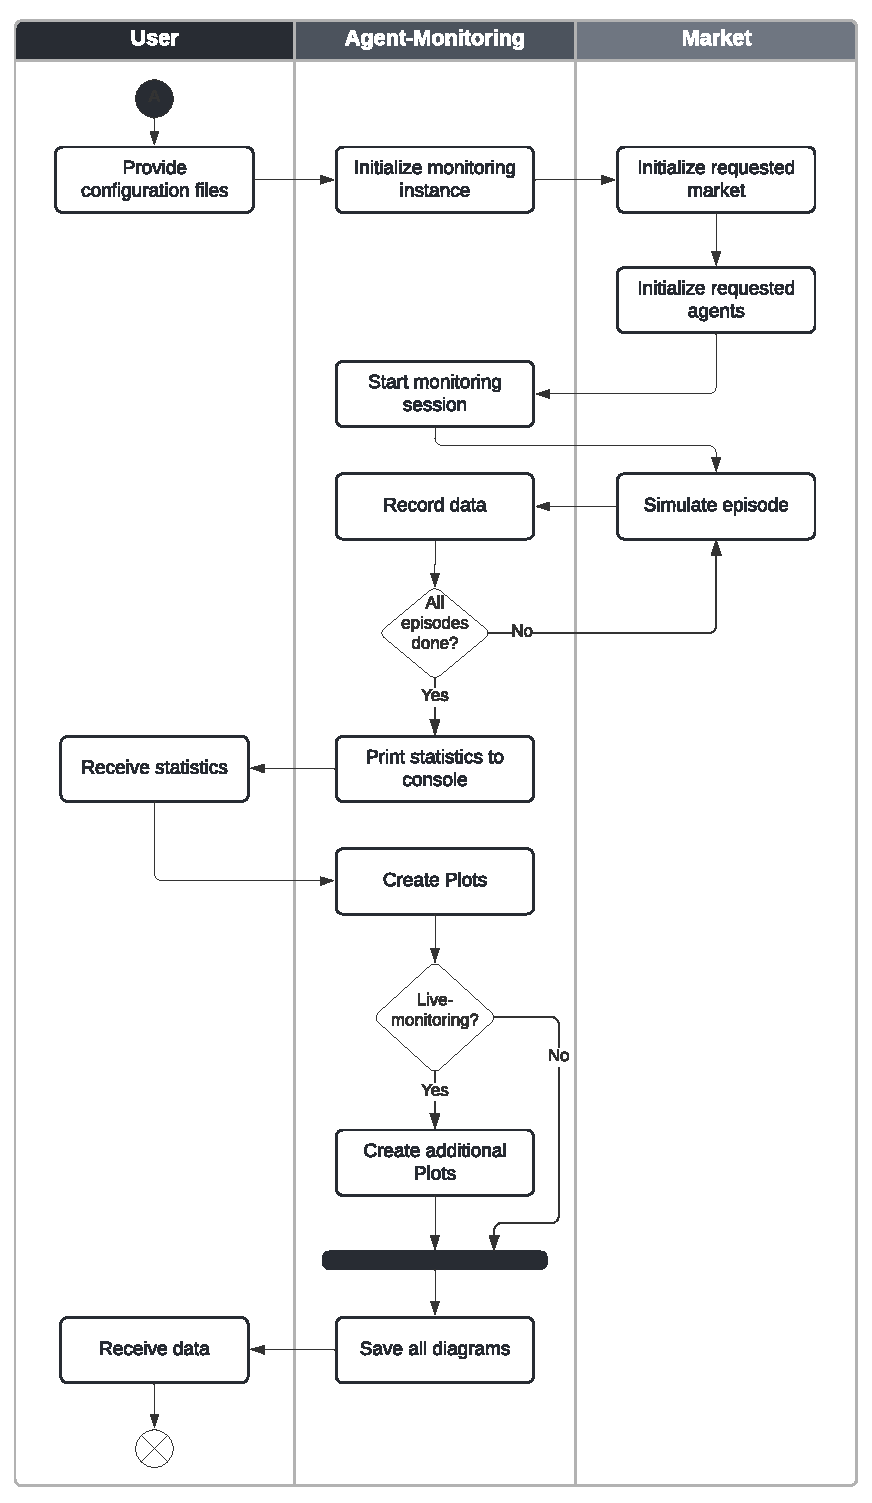
\includegraphics[height = 0.9\textheight]{images/swimlane_monitoring.pdf}\\
	\caption{The internal workflow when running an Agent-monitoring session. \Cref{tab:AllMetrics} lists the different types of diagrams created by both the Live- and Agent-Monitoring, and which of the recorded metrics they visualize.}\label{fig:SwimlaneMonitoring}
\end{figure}

The \emph{Agent-monitoring} is a highly configurable tool for monitoring and evaluating different combinations of agents and marketplaces. \Cref{fig:SwimlaneMonitoring} shows how the tool works internally.\todo{@Rainer @Alex: That diagram takes up a whole page - I would like to move it to the Appendix, is that `allowed', since it is quite integral to the tool?}

In addition to parameters provided to the marketplace and monitored agents, the following parameters can be used to configure the \emph{Agent-monitoring} tool itself:

\begin{enumerate}
	\item Episodes: This parameter decides how many independent simulations are run in sequence. At the start of each episode, the market state will be reset and randomized. Within an episode, the vendors run through a configurable amount of time steps, during each of which they set prices (depending on the chosen economy type, this can range from only one price for new items to three prices, including a rebuy price for used items) and a set number of customers interact with them.
	\item Plot interval: A number of diagram types enable the user to view averaged or aggregated data over a period of time. The plot interval parameter decides the size of these intervals. Smaller intervals mean more accurate but also more convoluted data points. Computational time also increases with a smaller interval size.
	\item Marketplace: Using this parameter, the user can set the marketplace on which the monitoring session will be run. Refer to \fullref{sec:MarketScenarios} for an explanation of the different available marketplaces.
	\item Separate markets: This parameter is a boolean flag that determines the way in which the monitoring session will handle the agents given by the user. If the flag is enabled, each agent will be initialized on a separate instance of the chosen marketplace, meaning that the agents will be monitored independent of each other. This functionality takes a lot longer than if the flag were disabled, as the whole marketplace is simulated once for each agent. While it may seem like the same results could be reached by simply starting multiple monitoring sessions with a different agent each, this is not the case. Using this flag instead, it is ensured that all agents get the exact same market states for each episode. By running multiple marketplaces in parallel using the \emph{separate markets} flag, we can match the simulations as closely as possible. The most prominent use case where this flag is enabled is during the Live-monitoring after a training session, where all intermediate models are being monitored on separate markets.

	      If the flag is disabled, the monitoring tool will initialize only one marketplace and set the passed agents to directly compete against each other on this marketplace. This functionality is most useful when monitoring only a single agent, trying to determine its specific strengths and weaknesses against certain opponents, as it will complete a lot faster than if the flag were enabled.
	\item Agents: Depending on the chosen marketplace, only a select number of agents can be chosen to be monitored, as each agent is built to interact with a specific type of marketplace. First off, all agents belong to one of the two major categories: \emph{Reinforcement-Learning agent} or \emph{Rule-Based agent} (for a more detailed overview see \fullref{sec:ExplainVendors}). Reinforcement-Learning agents can only be monitored on the marketplace type and market environment they were trained on, as these define the number of inputs and outputs the agent expects. Rule-Based agents can only be used on the marketplace type they were built for, as each of them makes assumptions about the number of prices they will need to set, but the market environment may be freely chosen. This leads to not all marketplace types having the same amount of Rule-Based vendors available. Following their importance for our simulation framework, the Linear Economy has the least and most often weakest vendors available, while the more refined competitors are most of the times only available as a version compatible with the Circular Economy with rebuy prices.
\end{enumerate}

During each episode and for each vendor, all market events are being recorded. At the end of the monitoring session, the collected data is evaluated in different visual formats. First of all, all data that would be available to see in the \emph{TensorBoard} during a training session is visualized using density plots. These plots can be used to compare the vendors in a more granular way, if for example the effect of a parameter on the customer's sell-back behaviour of used items should be tested. Another visualization that is created is a histogram containing the cumulative profits per episode for each agent, plotted against each other. This allows for a quick overview to see which agent had an overall better performance. One additional type of diagram is only created if the Agent-monitoring is run through the Live-monitoring tool: Violinplots. These plots, which are created for all data points available through TensorBoard (also see \Cref{tab:AllMetrics}), depict distributions using density curves, accentuating the minimum, maximum and median values. Violinplots are used by us to compare different training stages of an agent, as small policy changes can have great impact on these values. For exemplary Violinplots created after training, see \Cref{fig:SACDuopolyViolinPlots}.

Aside from monitoring after a training session, a common use case of the \emph{Agent-monitoring} tool is to test trained agents against competitors other than the ones it was trained against. This is done to test the agent's capacity to adapt to different circumstances, an important factor in deciding an agent's quality, as its competitors in the real market will differ from any it has encountered in training, due to the sheer vastness of options when it comes to dynamic pricing models available nowadays, see \fullref{sec:ExplainVendors}.

\subsection*{4.3.2 Exampleprinter}\label{subsec:Exampleprinter}

The \emph{Exampleprinter} is a tool meant for quickly evaluating a market scenario in-depth. When run, each action taken by the monitored agents is being recorded, in addition to market states and events such as the number of customers arriving and the amount of products thrown away. At the end of this quick simulation an animated overview diagram is created, which shows all actions and their consequences for each step in the simulation, see for example \Cref{fig:SACDuopolyExampleprinter17}. Due to the large amount of data that is being collected and visualized and the overhead would come with doing so for hundreds of episodes, we chose to disconnect this functionality from large-scale tools such as the Agent-monitoring. While the Agent-monitoring tool could be seen as a tool that imitates Macro-economic behaviour, simulating hundreds of days through hundreds of episodes, the Exampleprinter instead simulates only one day, recording and visualizing all data collected during that time.

\subsection*{4.3.3 Policyanalyser}\label{subsec:Policyanalyser}

The last tool we want to introduce is the \emph{Policyanalyser}. The \emph{Policyanalyser} is our only tool which does not simulate a market. Instead, the tool can be used to monitor an agent's reaction to different market states. The user can decide on up to two different features to give as an input, such as a competitor's new and refurbished prices, and the Policyanalyser will feed all possible input combinations to the agent and record its reactions. When initializing the \emph{Policyanalyser}, the user defines a number of parameters: The agent whose policy should be analysed, as well as the marketplace and the competitors that should be used, just as is done for all the other tools. Additionally, the user defines a \textbf{template market state}, a market state containing all values that are passed to the analysed agent, such as the number of items currently in circulation and the prices of competitors. Lastly, a list of \textbf{analysed features} needs to be provided, which defines one or two features of the template market state that should be varied. When the \emph{Policyanalyser} is run, these features are inserted into the template market state, overwriting the initial values and creating a new combination. This new market state is then passed on to the \texttt{policy}-method of the analysed agent (for an example policy, see \Cref{fig:PolicyRuleBasedStorageMinimizer})\todo{Just mention the seciton in Appendix}, and its reactions are recorded and visualized. See \bfref{subsec:ResultsPolicyanalyser} for use cases of this tool.

The \emph{Policyanalyser} is the monitoring tool which operates on the smallest scale out of all the tools we built for our framework. It allows users to define any market state they want and to then accurately monitor a vendor's reactions to changes to this specific state. While the tool can just as well be utilized to test new Rule-Based strategies, it is very much meant to be used as a way to understand Reinforcement-Learning agents better, as their policies are not immediately visible to the end-user and must therefore be discovered through tools such as the one's we built.
